%%%%%%%%%%%%%%%%%%%%%%%%%%%%%%%%%%%%%%%%%%%%%%%%%%%%%%%%%%%%%%%%%%%%%%%%%%%%%
%%% LaTeX-Rahmen fuer das Erstellen von englischen Bachelorarbeiten
%%%%%%%%%%%%%%%%%%%%%%%%%%%%%%%%%%%%%%%%%%%%%%%%%%%%%%%%%%%%%%%%%%%%%%%%%%%%%

%%%%%%%%%%%%%%%%%%%%%%%%%%%%%%%%%%%%%%%%%%%%%%%%%%%%%%%%%%%%%%%%%%%%%%%%%%%%%
%%% allgemeine Einstellungen
%%%%%%%%%%%%%%%%%%%%%%%%%%%%%%%%%%%%%%%%%%%%%%%%%%%%%%%%%%%%%%%%%%%%%%%%%%%%%

\documentclass[twoside,12pt,a4paper]{report}
%\usepackage{reportpage}
\usepackage{epsf}
\usepackage{graphics, graphicx}
\usepackage{latexsym}
\usepackage[margin=10pt,font=small,labelfont=bf]{caption}
\usepackage[utf8]{inputenc}

\textwidth 14cm
\textheight 22cm
\topmargin 0.0cm
\evensidemargin 1cm
\oddsidemargin 1cm
%\footskip 2cm
\parskip0.5explus0.1exminus0.1ex

% Kann von Student auch nach pers\"onlichem Geschmack ver\"andert werden.
\pagestyle{headings}

\sloppy

\begin{document}

%%%%%%%%%%%%%%%%%%%%%%%%%%%%%%%%%%%%%%%%%%%%%%%%%%%%%%%%%%%%%%%%%%%%%%%%%%%%
%%% Layout Title page
%%%%%%%%%%%%%%%%%%%%%%%%%%%%%%%%%%%%%%%%%%%%%%%%%%%%%%%%%%%%%%%%%%%%%%%%%%%%
 
\begin{titlepage}
 \begin{center}
  {\LARGE Eberhard Karls Universit\"at T\"ubingen}\\
  {\large Mathematisch-Naturwissenschaftliche Fakultät \\
Wilhelm-Schickard-Institut f\"ur Informatik\\[4cm]}
  {\huge Bachelor Thesis Bioinformatics\\[2cm]}
  {\Large\bf  Title of thesis\\[1.5cm]}
 {\large Name}\\[0.5cm]
Date\\[3cm]
\begin{center}
{\small\bf Reviewer}\\[0.5cm]
 {\large Name Reviewer}\\
  {\footnotesize Department of Computer Science\\
	University of T\"ubingen}
  \end{center}
	
\begin{center}
{\small\bf Supervisor}\\[0.5cm]
  {\large Name Supervisor}\\
  {\footnotesize Address\\
	University of T\"ubingen}\end{center}

  \end{center}
\end{titlepage}
%%%%%%%%%%%%%%%%%%%%%%%%%%%%%%%%%%%%%%%%%%%%%%%%%%%%%%%%%%%%%%%%%%%%%%%%%%%%
%%% Layout back of title page
%%%%%%%%%%%%%%%%%%%%%%%%%%%%%%%%%%%%%%%%%%%%%%%%%%%%%%%%%%%%%%%%%%%%%%%%%%%%

\thispagestyle{empty}
\vspace*{\fill}
\begin{minipage}{11.2cm}
\textbf{Name, first name:}\\
\emph{Title of thesis}\\ Bachelor Thesis Bioinformatics\\
Eberhard Karls Universit\"at T\"ubingen\\
Period: from-till
\end{minipage}
\newpage

%%%%%%%%%%%%%%%%%%%%%%%%%%%%%%%%%%%%%%%%%%%%%%%%%%%%%%%%%%%%%%%%%%%%%%%%%%%%

\pagenumbering{roman}
\setcounter{page}{1}

%%%%%%%%%%%%%%%%%%%%%%%%%%%%%%%%%%%%%%%%%%%%%%%%%%%%%%%%%%%%%%%%%%%%%%%%%%%%
%%% Page I: Abstract
%%%%%%%%%%%%%%%%%%%%%%%%%%%%%%%%%%%%%%%%%%%%%%%%%%%%%%%%%%%%%%%%%%%%%%%%%%%%


\section*{Abstract}

Write here your abstract.
\newpage
%%%%%%%%%%%%%%%%%%%%%%%%%%%%%%%%%%%%%%%%%%%%%%%%%%%%%%%%%%%%%%%%%%%%%%%%%%%%
%%% Page 2: Danksagung
%%%%%%%%%%%%%%%%%%%%%%%%%%%%%%%%%%%%%%%%%%%%%%%%%%%%%%%%%%%%%%%%%%%%%%%%%%%%
\section*{Acknowledgements}

Write here your acknowledgements.

\cleardoublepage

%%%%%%%%%%%%%%%%%%%%%%%%%%%%%%%%%%%%%%%%%%%%%%%%%%%%%%%%%%%%%%%%%%%%%%%%%%%%%
%%% Table of Contents
%%%%%%%%%%%%%%%%%%%%%%%%%%%%%%%%%%%%%%%%%%%%%%%%%%%%%%%%%%%%%%%%%%%%%%%%%%%%%

\renewcommand{\baselinestretch}{1.3}
\small\normalsize

\tableofcontents

\renewcommand{\baselinestretch}{1}
\small\normalsize

\cleardoublepage

%%%%%%%%%%%%%%%%%%%%%%%%%%%%%%%%%%%%%%%%%%%%%%%%%%%%%%%%%%%%%%%%%%%%%%%%%%%%%
%%% List of Figures
%%%%%%%%%%%%%%%%%%%%%%%%%%%%%%%%%%%%%%%%%%%%%%%%%%%%%%%%%%%%%%%%%%%%%%%%%%%%%

\renewcommand{\baselinestretch}{1.3}
\small\normalsize

\addcontentsline{toc}{chapter}{List of Figures}
\listoffigures

\renewcommand{\baselinestretch}{1}
\small\normalsize

\cleardoublepage

%%%%%%%%%%%%%%%%%%%%%%%%%%%%%%%%%%%%%%%%%%%%%%%%%%%%%%%%%%%%%%%%%%%%%%%%%%%%%
%%% List of tables
%%%%%%%%%%%%%%%%%%%%%%%%%%%%%%%%%%%%%%%%%%%%%%%%%%%%%%%%%%%%%%%%%%%%%%%%%%%%%

\renewcommand{\baselinestretch}{1.3}
\small\normalsize

\addcontentsline{toc}{chapter}{List of Tables}
\listoftables

\renewcommand{\baselinestretch}{1}
\small\normalsize

\cleardoublepage

%%%%%%%%%%%%%%%%%%%%%%%%%%%%%%%%%%%%%%%%%%%%%%%%%%%%%%%%%%%%%%%%%%%%%%%%%%%%%
%%% List of abbreviations
%%%%%%%%%%%%%%%%%%%%%%%%%%%%%%%%%%%%%%%%%%%%%%%%%%%%%%%%%%%%%%%%%%%%%%%%%%%%%

% can be removed
\addcontentsline{toc}{chapter}{List of Abbreviations}
\chapter*{List of Abbreviations\markboth{LIST OF ABBREVIATIONS}{LIST OF ABBREVIATIONS}}

\begin{tabbing}
\textbf{FACTOTUM}\hspace{1cm}\=Schrott\kill
\textbf{BLAST}\>Basic Local Alignment Search Tool \\
\textbf{...} \> ...\\
\end{tabbing}

\cleardoublepage

%%%%%%%%%%%%%%%%%%%%%%%%%%%%%%%%%%%%%%%%%%%%%%%%%%%%%%%%%%%%%%%%%%%%%%%%%%%%%
%%% Der Haupttext, ab hier mit arabischer Numerierung
%%% Mit \input{dateiname} werden die Dateien `dateiname' eingebunden
%%%%%%%%%%%%%%%%%%%%%%%%%%%%%%%%%%%%%%%%%%%%%%%%%%%%%%%%%%%%%%%%%%%%%%%%%%%%%

\pagenumbering{arabic}
\setcounter{page}{1}

%% Introduction
%%%%%%%%%%%%%%%%%%%%%%%%%%%%%%%%%%%%%%%%%%%%%%%%%%%%%%%%%%%%%%%%%%%%
% Einleitung
%%%%%%%%%%%%%%%%%%%%%%%%%%%%%%%%%%%%%%%%%%%%%%%%%%%%%%%%%%%%%%%%%%%%

\chapter{Introduction}\label{Introduction}

A good introduction is of utmost importance.


\medskip
Am Ende der Einleitung folgt ein Text so \"ahnlich wie (Nat\"urlich das folgende alles auf Englisch !!):

Die Arbeit gliedert sich dazu wie folgt: Die Grundlagen von ...
werden in Kapitel~\ref{Introduction} erarbeitet. 
...
Eine
Diskussion und ein kurzer Ausblick im
Kapitel~\ref{Discussion} beschlie{\ss}en diese Arbeit.

Bevor wir uns der Auswertung bzw. Bewertung der gewonnenen Prim\"ardaten zuwenden, wollen wir zun\"achst einige grundlegende Begriffe der deskriptiven Statistik wiederholen.
\section{Stichproben}

Grunds\"atzlich haben wir es bei Microarrayexpressionsdaten mit einer {\em Stichprobe} aus einer {\em Population (Grundgesamtheit)} zu tun.   
Wir bezeichnen nun im allgemeinen mit $X=\{x_1,x_2,\ldots,x_n\}$ die Beobachtungsdaten vom Umfang $n$. 
Diese Daten sollen mit statistischen Kenngr\"o\"sen beschrieben werden. Aus diesen will man m\"oglichst zuverl\"assig auf die zugrundeliegende Verteilung in der Grundgesamtheit schlie\"sen. Hierzu verwenden wir die {\bf Lage-} und {\bf Streuparameter}. Zun\"achst wenden wir uns aber der H\"aufigkeits- und Summenh\"aufigkeitsverteilung zu, die sowohl graphisch als auch numerisch einen Eindruck \"uber die Verteilung von $X$ bieten. Daf\"ur betrachten wir diskrete Verteilungen.

Gegeben sei eine Stichprobe $(X_1,X_2,\ldots,X_n)$. Eine Funktion $Z_n=Z(X_1,\ldots,X_n)$ heisst eine {\em Stichprobenfunktion}. Sie ist selber eine Zufallsgr\"o\"se.

\subsection{H\"aufigkeiten und Histogramm}
In $X$ trete der Wert $x_i$ genau $n_i$ mal auf, $i=1,2,\ldots m$. Dann ist $\sum_i n_i = n$. Der Quotient $n_i/n$ ist die {\em relative H\"aufigkeit} f\"ur das Eintreten des Ereignisses ``$X=x_i$''.
Die Menge der relativen H\"aufigkeiten $\{n_1/n,n_2/n,\ldots, n_m/n\}$ hei\"st {\em H\"aufigkeitsverteilung} von $X$. Ferner hei\"st die Menge $\{s_1,\ldots,s_m\}$ mit $s_i=\sum_{k=1}^{i}n_k/n$ die {\em Summenh\"aufigkeitsverteilung} von $X$.

F\"ur die graphische Darstellung der H\"aufigkeitsverteilung wird das {\em Histogramm} (s. Abb.~) gew\"ahlt. f\"ur die Summenh\"aufigkeitsverteilung die {\em Treppenfunktion}.

%
\subsection{Wichtige Verteilungen}

\subsubsection{Die Normalverteilung}
Die Dichte der Normalverteilung ist gegeben durch
\begin{equation}\label{dichtenormal}
g(x) = \frac{1}{2\pi\sigma}\cdot e^{-\frac{(x-\mu)^2}{2\sigma^2}}
\end{equation}
wobei $\mu$ (Lage) der Mittelwert und $\sigma$ (Breite) die Standardabweichung der Normalverteilung ist. 
Durch die $z$-Transformation l\"asst sich die Normalverteilung auf die Standardnormalverteilung mit $\mu=0$ und $\sigma=1$ transformieren.

Die Normalverteilung bildet die Basis fast der gesamten statistischen Theorie. \footnote{ 
``Everyone believes in the normal law, the experimenters because they imagine it is a mathematical theorem, and the mathematicians because they think it is an experimental fact.'' (Gabriel Lippman, in Poincar\'e's Calcul de probabilit\'es, 1896)}. Auch bei der Analyse der Microarraydaten werden wir sehr oft von der Annahme der Normalverteilung Gebrauch machen. Allerdings sollten wir uns klarmachen, dass  rein experimentell zahlreiche Untersuchungen gezeigt haben, dass die echten Fehler selten, wenn \"uberhaupt normal verteilt sind.


\section{Sch\"atzung von Parametern}
Allgemein erhofft man sich beim Ziehen einer Stichprobe, einen unbekannten Parameter $\gamma$ der Grundgesamtheit, z.B. den Mittelwert, aus der Stichprobe zu sch\"atzen.
\subsection{Eigenschaften von Punktsch\"atzungen}


\cleardoublepage

%% 
%%%%%%%%%%%%%%%%%%%%%%%%%%%%%%%%%%%%%%%%%%%%%%%%%%%%%%%%%%%%%%%%%%%%
% Grundlagen
%%%%%%%%%%%%%%%%%%%%%%%%%%%%%%%%%%%%%%%%%%%%%%%%%%%%%%%%%%%%%%%%%%%%

\chapter{Material and Methods}
  \label{MatMet}

\noindent
In this chapter ...

\section{Title of section}
  \label{Abschnittslabel} 

BlaBlaBla ...

\subsection{Title of subsection}
  \label{Unterabschnittslabel}

BlaBlaBla ...

Zum Einbinden einer Abbildung mittels `pdf-Datei' in ein
\LaTeX-Dokument benutzt man folgenden \LaTeX-Code:

\begin{verbatim}
\begin{figure}[htb]
     \centerline{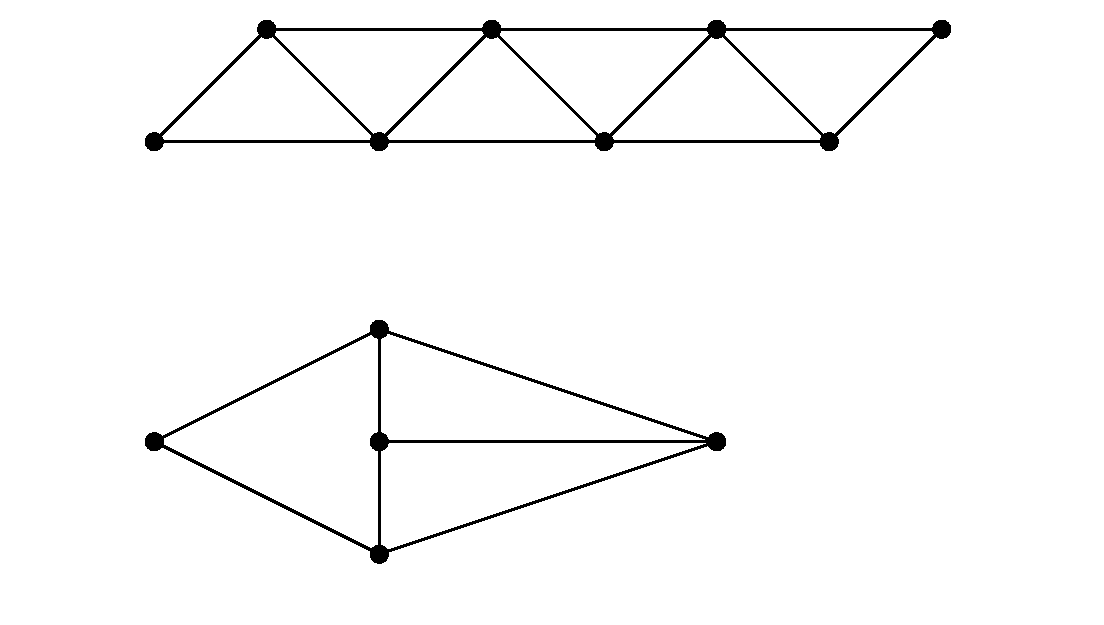
\includegraphics{figures/chordal.pdf}}
  \caption{Chordale Graphen}
  \label{chordal}
\end{figure}
\end{verbatim}

\begin{figure}[htb]
     \centerline{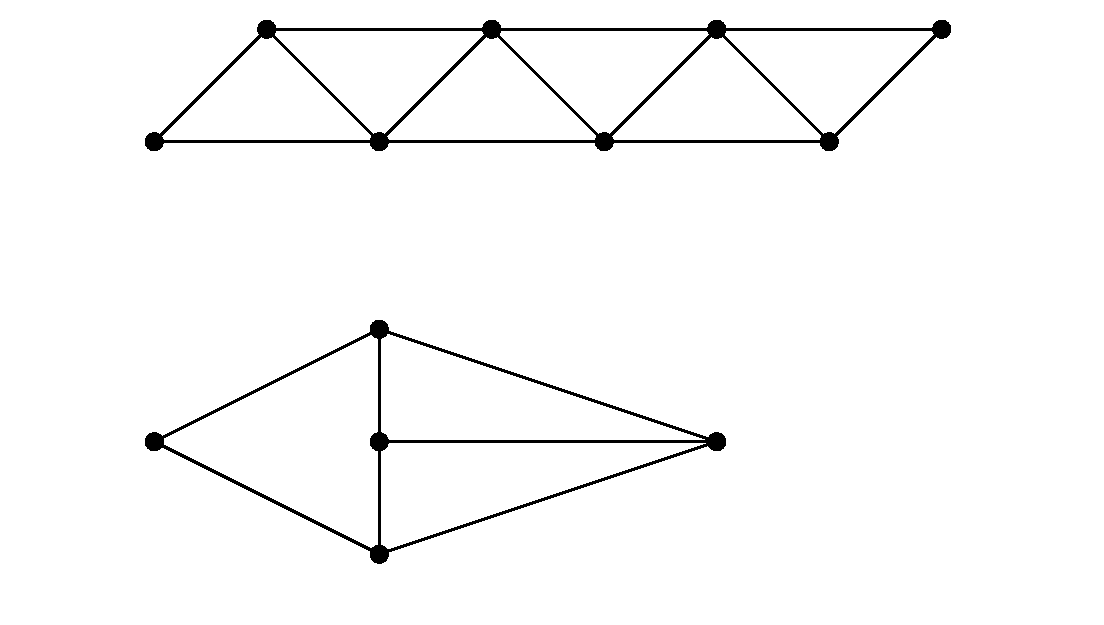
\includegraphics{figures/chordal.pdf}}
  \caption{Chordal Graphs}
  \label{chordal}
\end{figure}

Abbildung~\ref{chordal} zeigt ...

Tabellen k\"onnen wie folgt erstellt werden:

{
\renewcommand{\baselinestretch}{0.9} 
\normalsize
\begin{table}[htb]
\begin{tabular}{|p{2.7cm}||l|c|r|}
\hline
    \textbf{Spalte 1} 
  & \textbf{Spalte 2} 
  & \textbf{Spalte 3} 
  & \textbf{Spalte 4} \\
  \hline\hline
  xxx1111
  & xxxxxxx2222222
  & xxxxxx333333 
  & xxxxxxxxxx444444 \\
  \hline
    ...
  & ...
  & ...
  & ...\\
  \hline
\end{tabular}
  \caption[Diese Kurzcaption ist fuer das Tabellenverzeichnis]{Beispieltabelle mit einer langen Legende, damit man sieht, dass in der Legende der Zeilenabstand verringert wurde. Ausserdem soll auch der Font etwas kleiner gew\"ahlt werden. So sieht die ganze Umgebung kompakter aus.}
  \label{tabelle-1}
\end{table}
}

\noindent
Eine Aufz\"ahlung geht wie folgt:
\begin{itemize}
\item ...
\item ...
\end{itemize}
Eine numerierte Aufz\"ahlung:
\begin{enumerate}
\item ...
\item ...
\end{enumerate}

Betonungen sollen \emph{kursiv} gedruckt werden. 
\textbf{Fettdruck} ist auch m\"oglich.

Referenzen: \cite{SaaSchTue97,TueConSaa96ismis,SchTueSaa98preprint}

\cleardoublepage

%%
%%%%%%%%%%%%%%%%%%%%%%%%%%%%%%%%%%%%%%%%%%%%%%%%%%%%%%%%%%%%%%%%%%%%
% Diskussion und Ausblick
%%%%%%%%%%%%%%%%%%%%%%%%%%%%%%%%%%%%%%%%%%%%%%%%%%%%%%%%%%%%%%%%%%%%

\chapter{Discussion and Outlook}
  \label{Discussion}

Take your time for writing the discussion, it is the most important chapter of your thesis.

At least 4-5 pages.

\bigskip
Outlook can become an extra chapter.

\cleardoublepage


%%%%%%%%%%%%%%%%%%%%%%%%%%%%%%%%%%%%%%%%%%%%%%%%%%%%%%%%%%%%%%%%%%%%%%%%%%%%%
%%% Bibliographie
%%%%%%%%%%%%%%%%%%%%%%%%%%%%%%%%%%%%%%%%%%%%%%%%%%%%%%%%%%%%%%%%%%%%%%%%%%%%%

\addcontentsline{toc}{chapter}{Bibliography}

\bibliographystyle{alpha}
\bibliography{mylit}
%% Obige Anweisung legt fest, dass BibTeX-Datei `mylit.bib' verwendet
%% wird. Hier koennen mehrere Dateinamen mit Kommata getrennt aufgelistet
%% werden.

\cleardoublepage

%%%%%%%%%%%%%%%%%%%%%%%%%%%%%%%%%%%%%%%%%%%%%%%%%%%%%%%%%%%%%%%%%%%%%%%%%%%%%
%%% Erklaerung
%%%%%%%%%%%%%%%%%%%%%%%%%%%%%%%%%%%%%%%%%%%%%%%%%%%%%%%%%%%%%%%%%%%%%%%%%%%%%
\thispagestyle{empty}
\section*{Selbst\"andigkeitserkl\"arung}

Hiermit versichere ich, dass ich die vorliegende Bachelorarbeit 
selbst\"andig und nur mit den angegebenen Hilfsmitteln angefertigt habe und dass alle Stellen, die dem Wortlaut oder dem 
Sinne nach anderen Werken entnommen sind, durch Angaben von Quellen als 
Entlehnung kenntlich gemacht worden sind. 
Diese Bachelorarbeit wurde in gleicher oder \"ahnlicher Form in keinem anderen 
Studiengang als Pr\"ufungsleistung vorgelegt. 

\vskip 3cm

Ort, Datum	\hfill Unterschrift \hfill 


%%% Ende
%%%%%%%%%%%%%%%%%%%%%%%%%%%%%%%%%%%%%%%%%%%%%%%%%%%%%%%%%%%%%%%%%%%%%%%%%%%%%

\end{document}

